\documentclass[main.tex]{subfiles} 
\begin{document}

\section{VIDEO COMPREHENSION SCORE (VCS): A METRIC FOR LONG-FORM VIDEO DESCRIPTION EVALUATION}

\subsection{INTRODUCTION}

Recent advancements in Large Video Language Models (LVLMs) \cite{Yuan2025Tarsier2,Shen2025LongVU,Ataallah2024Goldfish,Chen2025LongVILA} have enhanced automated video comprehension, enabling long-form description generation from long videos. However, exploratory analysis on long videos reveals that LVLMs frequently (i) miss global narrative structure, (ii) fail to capture local events, and (iii) fail to establish temporal connections while hallucinating content. These gaps indicate LVLMs lack true video comprehension, raising the question: how can we evaluate models' video comprehension? Current benchmarks utilize question-answering formats \cite{wu2024longvideobench,ataallah2024infinibench,nagrani2025neptune} or short-form description comparisons for short videos \cite{wyzs:24,chen:acl11,ZhXuCoAAAI18}, both inadequate to evaluate models' true video comprehension ability. Evaluating genuine comprehension demands shifting to a methodology that processes long or complex videos and requires models to generate long-form descriptions. This approach renders superficial frame-level analysis insufficient, compelling models to instead generate outputs that capture global narrative structure, detail specific local events, and establish their temporal relationships. The quality of these generated descriptions can then be evaluated against the source video or human-written descriptions.

Description-based evaluation methods fall into four categories, each struggling with fundamental aspects of long-form evaluation. N-gram metrics such as BLEU \cite{p:02}, METEOR \cite{bl:05}, CIDEr \cite{v:15}, and ROUGE \cite{l:04} rely on lexical overlap, which not only unfairly penalizes legitimate paraphrases but also rewards superficial word-level matches between descriptions with entirely different global narratives. Embedding-based metrics like BERTScore \cite{z:20} and SBERT \cite{r:19} address lexical limitations through semantic similarity but overlook chronological alignment and local fine-grained details, allowing misordered events and subtle errors to remain undetected. Multimodal metrics such as EMScore \cite{syxl:22} enable direct comparison against source video content but struggle with long videos and long-form descriptions. LLM-based metrics such as CLAIR \cite{chan:23} and AutoDQ \cite{wyzs:24} provide deeper insights but often do not evaluate the chronology of events while suffering from consistency issues.

To address these limitations, we introduce VCS with three components:
\begin{enumerate}
\item \textbf{Global Alignment Score (GAS)}: Measures global thematic alignment.
\item \textbf{Local Alignment Score (LAS)}: Assesses local semantic alignment.
\item \textbf{Narrative Alignment Score (NAS)}: Evaluates chronological alignment using configurable Local Narrative Tolerance (LNT).
\end{enumerate}

VCS combines these three components to provide comprehensive evaluation: GAS and LAS form the Semantic Alignment Score (SAS), which integrates with NAS to produce the final VCS score. We also present VCS$_{\text{short}}$, which applies the same framework to short-form descriptions.

To evaluate VCS, we need datasets of long-form video descriptions paired with quality assessments—but no such datasets exist. Although creating a human-annotated dataset with quality ratings would be ideal, it is impractical: producing and reviewing long-form descriptions is costly and time-consuming, and annotator agreement declines sharply as description length increases. We therefore constructed a large-scale synthetic dataset from the MPII Movie Description Dataset \cite{rohrbach2015dataset} via ChatGPT-4o. From this dataset, we derived two test sets: a Corruption Detection Test Set to evaluate VCS ability to distinguish valid variations from invalid corruptions, and a Cross-Author Consistency Test Set to assess robustness across different authorial styles. VCS consistently outperforms traditional metrics on corruption detection tasks. To assess human correlation, we evaluate VCS$_{\text{short}}$ on VATEX-EVAL \cite{syxl:22}, where it achieves state-of-the-art results. These results demonstrate VCS effectiveness for robust evaluation of both long-form and short-form video descriptions.

Our primary contributions include:
\begin{itemize}
\item A robust metric (VCS) for both long-form and short-form video descriptions.
\item Configurable LNT and chunk size parameters to govern chronological strictness and comparison granularity.
\end{itemize}

\subsection{RELATED WORK}

Traditional n-gram-based metrics such as BLEU \cite{p:02}, ROUGE \cite{l:04}, and METEOR \cite{bl:05} evaluate text generation through lexical overlap and local word order. BLEU measures n-gram precision with brevity penalties, capturing local ordering but missing event-level chronology and struggling with expressive variability. ROUGE variants compute precision, recall, and F1-scores: ROUGE-N evaluates n-gram overlap, ROUGE-L computes Longest Common Subsequence at summary-level, and ROUGE-Lsum calculates sentence-level LCS by splitting at newlines. While preserving sequential information, they miss event-level chronology and remain sensitive to expressive variability. METEOR addresses expressive variability via synonyms and stems, computing recall-weighted F-scores with fragmentation penalties, but similarly misses event-level chronology. CIDEr \cite{v:15} uses consensus-based TF-IDF weighting across multiple references but proves impractical for long-form descriptions due to labor-intensive annotation. SPICE \cite{afjg:16} evaluates semantic propositions using graph overlaps, effectively handling paraphrasing; however, being designed for static images, it cannot be directly applied to videos and neglects narrative chronology critical for video descriptions.

Embedding-based metrics compare texts in semantic vector spaces, leveraging pretrained models to capture semantic similarity beyond lexical matches. BERTScore computes token-level similarity using contextualized BERT embeddings, aggregating optimal alignments into precision, recall, and F1-scores, while SBERT employs siamese networks with mean-pooling for sentence-level embeddings, but both address expressive variability by recognizing paraphrases yet are constrained by limited context windows, complicating their direct application to long-form descriptions. Recent decoder-based models such as NV-Embed-v2 \cite{l:24}, Linq-Embed-Mistral, SFR-Embedding-Mistral, and Jasper and Stella leverage autoregressive LLM architectures with bidirectional attention, offering significantly larger context windows and robust global embeddings, excelling at paragraph-level semantic assessments. However, reliance on global embeddings and cosine similarity overlooks local content alignment, detailed information accuracy, and chronological alignment.

Multimodal embedding metrics like EMScore \cite{syxl:22} and PAC-S employ vision-language models such as CLIP \cite{Radford2021LearningTV} to evaluate semantic alignment between visuals and generated captions, addressing expressive variability through direct image-caption comparison, thus bypassing reference captions. EMScore computes video-caption similarity through dual-level matching: coarse-grained alignment between video and caption embeddings, and fine-grained matching between frames and words, calculating precision, recall, and F1-scores via cosine similarity. PAC-S fine-tunes CLIP through positive-augmented contrastive learning with synthetic image-text pairs, then computes cosine similarity scores from the enhanced model. Despite their effectiveness in short-form descriptions, these metrics face computational challenges and methodological limitations when scaling to long-form descriptions.

Recent evaluation approaches increasingly leverage Large Language Models (LLMs), categorized into component-based and holistic judge methods. Component-based methods such as AutoDQ \cite{wyzs:24} extract events from descriptions using ChatGPT, then compute precision and recall through entailment analysis comparing extracted events between texts, while VAD-Score employs LLMs for semantic extraction and scoring of events, subjects, and objects, effectively addressing expressive variability but missing chronological evaluation. Holistic methods such as CapScore prompt GPT-4 to score caption similarity and quality, CapArena-Auto Score uses GPT-4o for pairwise evaluation battles, and CLAIR \cite{chan:23} employs zero-shot prompting for similarity scores with interpretable reasoning. However, these methods suffer from ambiguity in score calibration, sensitivity to prompting nuances, consistency issues across model versions, limited interpretability, and practical constraints including reproducibility and cost.

\subsection{METHODOLOGY}
\label{sec:methodology_vcs}

\begin{figure*}[t]
\centering
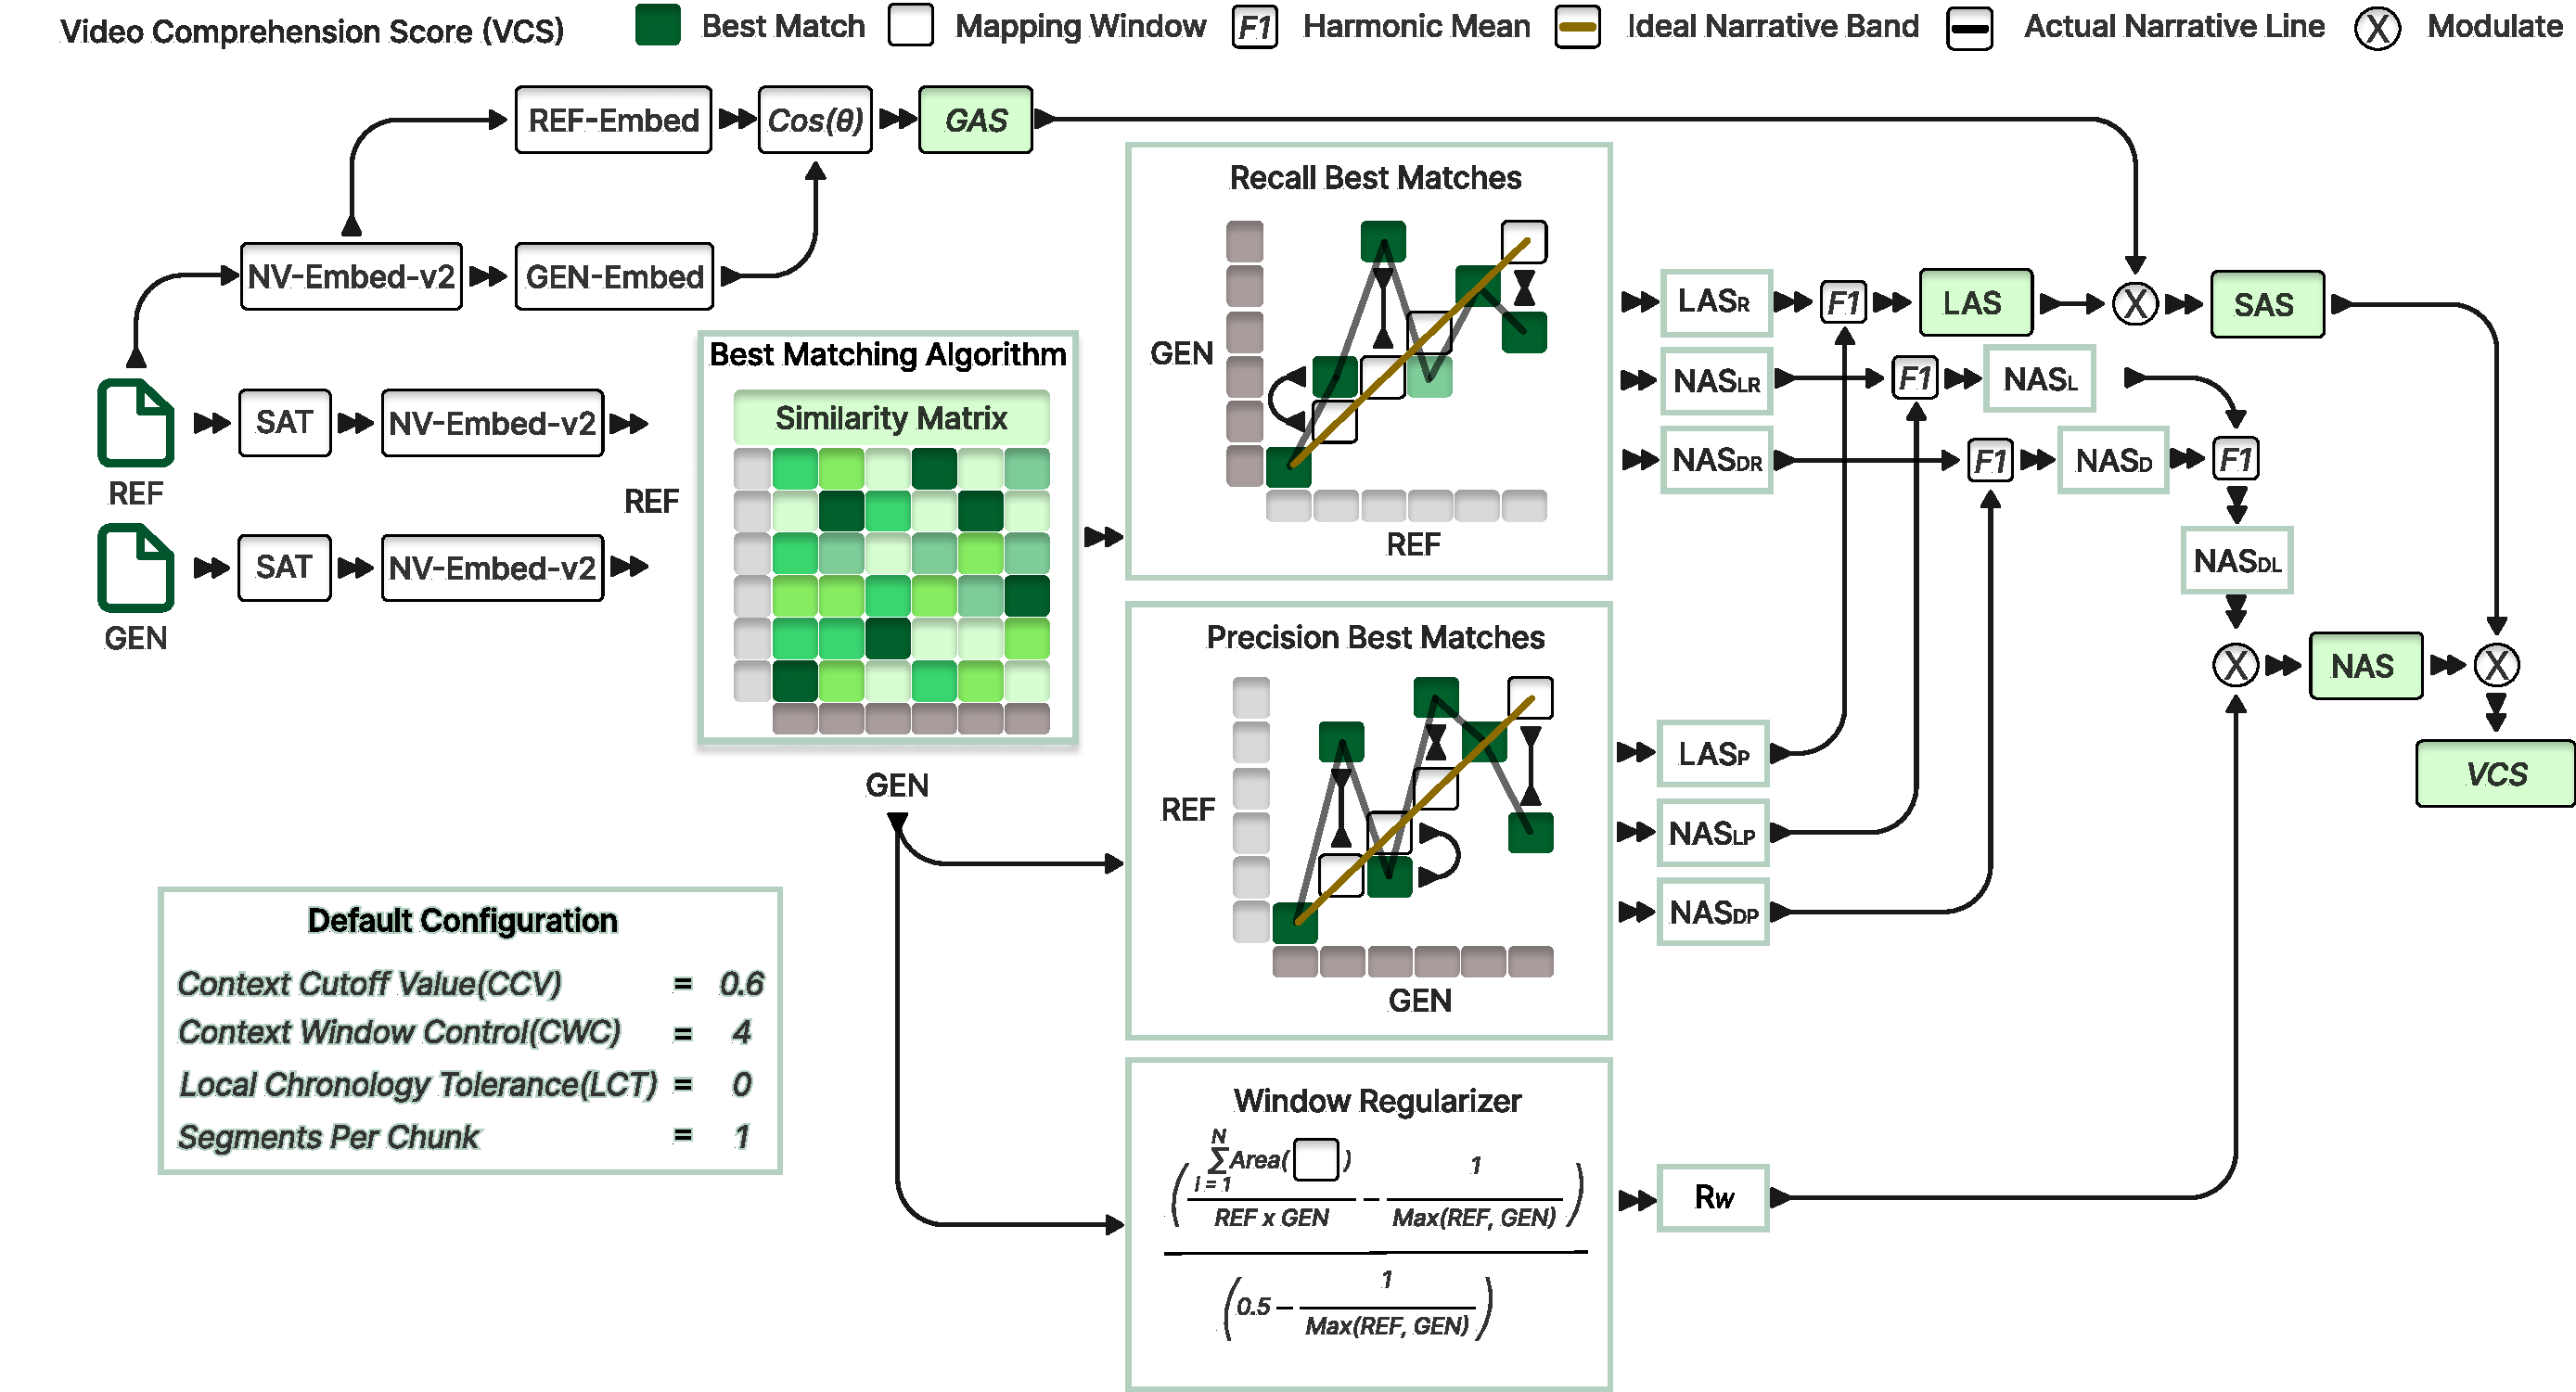
\includegraphics[width=0.8\textwidth]{images/VCS.pdf}
\caption{VCS Pipeline. The VCS assesses video descriptions by comparing a reference text ($T_{ref}$) with a model-generated text ($T_{gen}$). Both texts are initially segmented by SaT and embedded via NV-Embed-v2. The Global Alignment Score (GAS) is computed from the full text embeddings. For localized analysis, texts are chunked and embedded, forming a similarity matrix. From this, precision and recall-oriented best matches yield the Local Alignment Score (LAS)—the harmonic mean of $LAS_P$ (precision) and $LAS_R$ (recall). The Narrative Alignment Score (NAS) incorporates distance-based ($NAS_D$) and line-based ($NAS_L$) assessments. $NAS_D$ and $NAS_L$ are harmonic means of their respective precision and recall components. A Window Regularizer ($R_W$) refines the NAS. The Semantic Alignment Score (SAS) is derived by modulating GAS with LAS. The final VCS results from modulating the smaller of SAS and the regularized NAS with the larger.}
\label{fig:vcs-architecture}
\end{figure*}

Figure~\ref{fig:vcs-architecture} shows the VCS pipeline, which computes semantic and narrative alignment between reference and generated descriptions to achieve comprehensive long-form video description evaluation.

\subsubsection{Global Alignment Score (GAS)}
VCS computes GAS to capture global thematic alignment between reference and generated descriptions. Given input texts $T_{ref}$ and $T_{gen}$, we encode each description using NV-Embed-v2. The GAS is computed as:

\begin{equation} \label{eq:gas_revised}
\text{GAS} = \frac{\mathbf{E}_{ref} \cdot \mathbf{E}_{gen}}{\|\mathbf{E}_{ref}\| \|\mathbf{E}_{gen}\|}
\end{equation}

\subsubsection{Text Preprocessing for Chunk-Level Analysis}
However, GAS lacks sensitivity to fine-grained details and chronological consistency. To enable fine-grained analysis, VCS applies punctuation removal and Segment Any Text (SaT)~\cite{frohmann-etal-2024-segment} segmentation to $T_{ref}$ and $T_{gen}$, producing semantic segments $S_{ref}$ and $S_{gen}$. We group $k$ consecutive segments into chunks $C_{ref} = \{c_1^{ref}, \ldots, c_{N_{ref}}^{ref}\}$ and $C_{gen} = \{c_1^{gen}, \ldots, c_{N_{gen}}^{gen}\}$, embedded using NV-Embed-v2 to yield matrices $\mathbf{E}_{C_{ref}} \in \mathbb{R}^{N_{ref} \times D}$ and $\mathbf{E}_{C_{gen}} \in \mathbb{R}^{N_{gen} \times D}$.

\subsubsection{Defining Mapping Windows}
Before establishing chunk correspondences for fine-grained assessment, VCS constructs a similarity matrix to enable optimal alignments. Using $\mathbf{E}_{C_{ref}}$ and $\mathbf{E}_{C_{gen}}$, we compute similarity matrix:
\begin{equation}
\mathbf{S} \in \mathbb{R}^{N_{ref} \times N_{gen}} \text{ where } S_{i,j} = \cos(\mathbf{E}_{C_{ref}}[i], \mathbf{E}_{C_{gen}}[j])
\end{equation}
which represents the cosine similarity between the $i$-th reference chunk and $j$-th generated chunk.

However, before selecting the best match for each chunk, VCS defines Mapping Windows (MW) that constrain the search space within this similarity matrix. This concept stems from empirical observations: when computing pairwise chunk embeddings between identical long-form descriptions, the resulting similarity matrix exhibits a clear diagonal structure where $C_1^{ref}$ maps to $C_1^{gen}$, $C_2^{ref}$ maps to $C_2^{gen}$, and so on, with this diagonal pattern stretching or compressing proportionally in brevity or verbosity cases. Hence, for given chunk counts $N_{ref}$ and $N_{gen}$, we define this diagonal search space and call it Mapping Windows—regions where each chunk should ideally map.

VCS identifies the longer sequence as $\max(N_{ref}, N_{gen})$ and the shorter sequence as $\min(N_{ref}, N_{gen})$. We compute slope $s = \text{longer}/\text{shorter}$ and base window height $h_{mw} = \lceil s \rceil$. The algorithm creates direct windows by mapping each position $i$ in the shorter sequence to a window of height $h_{mw}$ in the longer sequence, spanning range $[\lfloor i \cdot s \rfloor, \min(\lfloor i \cdot s \rfloor + h_{mw}, \text{longer}))$ with proportional scaling. Reverse windows invert this mapping: for each position in the longer sequence, we determine which positions in the shorter sequence include it. VCS assigns Precision Windows ($MW_p$) and Recall Windows ($MW_r$) based on sequence direction: when $N_{ref} \geq N_{gen}$, precision uses direct windows and recall uses reverse windows; otherwise, assignments are reversed.

\subsubsection{Best Matching Algorithm}
Having established Mapping Windows within the similarity matrix $\mathbf{S}$, VCS pairs each generated chunk with its best reference counterpart, and vice versa. Naively selecting the highest-similarity reference for each generated chunk leads to semantic collision and semantic ambiguity. Semantic collision occurs when a single chunk exhibits identical similarity to multiple counterparts, while semantic ambiguity arises when a chunk achieves nearly equal similarity with multiple candidates. Both issues stem from repeated events or superficial lexical overlap, obscuring true narrative counterparts.

VCS resolves these issues through a Best-Matching Algorithm that combines adaptive context filtering with mapping-window constraints. Adaptive context filtering first determines a candidate set around the maximum similarity rather than committing immediately to the top score. Two user-defined parameters control this process: the context cutoff $\tau_{ctx}$ (default 0.6) and the context window control $k_{ctx}$ (default 4). Similarities below the cutoff receive no context expansion, while those above it define a context window whose width is computed as $w_{ctx} = \frac{(1-\tau_{ctx})-(1-s_{max})}{s_{max} \cdot k_{ctx}}$,

where $s_{max}$ is the maximum similarity for the chunk. All candidates within $s_{max} - w_{ctx}$ enter the pool for selection. Mapping-window constraints then enforce temporal alignment: among the candidate matches, the algorithm chooses the chunk closest to the mapping-window boundary of the target chunk, breaking ties by similarity. When $s_{max}$ falls below the cutoff, no context expansion occurs, and ties are resolved purely by distance from the mapping-window boundary.

This combination mitigates both collision and ambiguity. Executing this procedure for each generated chunk and each reference chunk yields precision best matches $M_P = \{(C_j^{gen}, C_{i^*}^{ref})\}$ and recall best matches $M_R = \{(C_i^{ref}, C_{j^*}^{gen})\}$.

\subsubsection{Local Alignment Score (LAS)}
Having obtained the correspondence sets $M_P$ and $M_R$ from the Best-Matching Algorithm, VCS computes the LAS by averaging cosine similarities of matched chunk pairs. The precision component $LAS_P$ evaluates how well generated text aligns with reference text, while recall component $LAS_R$ evaluates the reverse. LAS is their harmonic mean $LAS = \frac{2 \cdot LAS_P \cdot LAS_R}{LAS_P + LAS_R}$.

\subsubsection{Narrative Alignment Score (NAS)}
However, LAS remains insensitive to chronological ordering and exhibits limited sensitivity to missing or extra content. While LAS performs local semantic alignment and can detect content variations, its reliance on semantic similarity averaging means that even weak semantic matches contribute to the overall score, reducing its ability to strongly penalize missing or extraneous content. To mitigate both limitations, VCS introduces NAS that evaluates chronological consistency while enhancing sensitivity to content gaps and additions through narrative alignment assessment. NAS comprises four components: Distance-based NAS ($NAS_D$), Line-based NAS ($NAS_L$), a window regularizer, and the user-controlled Local Narrative Tolerance (LNT) parameter.

\subsubsection{Defining Local Narrative Tolerance (LNT)}
Before assessing narrative alignment, VCS defines a user-controlled parameter called LNT. This concept stems from the observation that video narratives often permit multiple valid orderings and descriptive variations where temporally adjacent or concurrent events can be described in different sequences and detail levels without compromising narrative coherence. Complex video scenes frequently contain multiple actors and objects performing concurrent actions, where these details can be expressed in multiple valid orders and varying descriptive granularity—from highly detailed to moderate to sparse descriptions. To accommodate this inherent flexibility, VCS employs LNT as a tolerance parameter that defines acceptable deviation from strict chronological order and descriptive consistency, allowing higher LNT values to provide tolerance for both narrative reordering and descriptive variability when dense descriptions describe scenes with slightly different detail levels.

\subsubsection{Distance-based NAS ($NAS_D$)}
Given the one-to-one correspondences $M_P$ (generated$\rightarrow$reference) and $M_R$ (reference$\rightarrow$generated) returned by the Best-Matching Algorithm, $NAS_D$ penalises every match whose index falls outside its Mapping Window. Let $y$ denote the length of the timeline being evaluated (reference when computing precision, generated when computing recall) and $\ell$ be the total number of Mapping Windows in that orientation.

\paragraph{Local Chronology Tolerance (LCT)}
The auxiliary window height that defines the tolerance zone is $h_{LCT} = \left\lceil \frac{y}{x} \right\rceil - \mathbf{1}[y > x \land 0 < \frac{y}{x} - \left\lfloor \frac{y}{x} \right\rfloor \leq 0.5]$
where $x$ is the length of the opposite timeline. Thus $h_{LCT}$ is the Mapping-Window height (ceiling of the length ratio) but drops by one row when the longer/shorter ratio's fractional part lies in $(0, 0.5]$.

A user-controlled multiplier $\tau_{LCT} \geq 0$ expands each Mapping Window by $\tau_{LCT} \cdot h_{LCT}$ rows on both sides. Any match whose vertical distance from the window boundary is $\leq \tau_{LCT} \cdot h_{LCT}$ is treated as chronologically acceptable and incurs no penalty.

\paragraph{Per-chunk distance penalty}
For a match located at index $k$ with original Mapping Window $[s, e)$, the distance penalty is $d(k) = s - k$ if $k < s$ and $d(k) = k - (e - 1)$ if $k \geq e$. After applying LCT, the effective penalty for that chunk is $p(k) = \frac{\max(0, d(k) - \tau_{LCT} \cdot h_{LCT})}{y}$, and $p(k) = 0$ if the chunk was already inside its window.

\paragraph{Sequence-level normalisation}
The actual total penalty $P_{total} = \sum_{j=1}^{\ell} p(k_j)$ and maximum possible penalty $P_{\max} = \frac{1}{y} \sum_{j=1}^{\ell} \max(s_j, y - e_j)$ (obtained by pushing every match to whichever timeline edge is further away) yield the orientation-specific scores $NAS_{D,prec} = 1 - \frac{P_{total,prec}}{P_{\max,prec}}$ and $NAS_{D,rec} = 1 - \frac{P_{total,rec}}{P_{\max,rec}}$.

\paragraph{Bidirectional fusion}
Finally, $NAS_D$ combines both views through the harmonic mean $NAS_D = \frac{2 \cdot NAS_{D,prec} \cdot NAS_{D,rec}}{NAS_{D,prec} + NAS_{D,rec}}$.

\subsubsection{Line-based NAS ($NAS_L$)}

\paragraph{Ideal narrative-line band}
Let the Mapping Windows be $W_i = [a_i, b_i)$ for $i = 1, \ldots, n$ with $x_i = i$. The shortest and longest feasible path lengths:
\begin{equation}
L_{\min} = \min_{y_i \in W_i} \sum_{i=1}^{n-1} \sqrt{(x_{i+1} - x_i)^2 + (y_{i+1} - y_i)^2}, \quad L_{\max} = \max_{y_i \in W_i} \sum_{i=1}^{n-1} \sqrt{(x_{i+1} - x_i)^2 + (y_{i+1} - y_i)^2}
\end{equation}
are obtained by dynamic-programming over consecutive windows: every candidate $y_{i+1}$ is relaxed from every candidate $y_i$ with edge-weight $\sqrt{1^2 + (y_{i+1} - y_i)^2}$. Tracing predecessors yields a floor path of length $L_{\min}$ and a ceil path of length $L_{\max}$.

The successive vertical differences $\Delta y_i^{\text{floor}}$ along the floor path are cached in a map $\text{DY}_{\text{floor}}[x_i] = \Delta y_i^{\text{floor}}$; they later cap oversized jumps when Local Chronology Tolerance (LCT) is enabled.

\paragraph{Local Chronology Tolerance (LCT)}
Let $L_s$ be the length of the source timeline (x-axis) and $L_t$ the length of the target timeline (y-axis). Define the base Mapping-Window height $h_{mw} = \left\lceil \frac{L_t}{L_s} \right\rceil$.
From this, the LCT window $\omega_0$ and its expanded version $\omega_{LCT}$ are defined where $\rho = L_t/L_s - \lfloor L_t/L_s \rfloor$ and $\tau_{LCT} \in \mathbb{N}_{\geq 0}$ is user-set:
\begin{align}
\omega_0 &= \begin{cases}
h_{mw}, & L_t \leq L_s, \\
2h_{mw} - 2, & L_t > L_s \text{ and } 0 < \rho \leq 0.5, \\
2h_{mw} - 1, & L_t > L_s \text{ and } \rho > 0.5,
\end{cases} \\
\omega_{LCT} &= \omega_0 + \begin{cases}
h_{mw} \tau_{LCT}, & L_t \leq L_s, \\
(h_{mw} - 1) \tau_{LCT}, & 0 < \rho \leq 0.5, \\
h_{mw} \tau_{LCT}, & \rho > 0.5
\end{cases}
\end{align}

\paragraph{Actual narrative-line length}
The aligned points are sorted by the source index. For consecutive pairs $(x_i, y_i)$, $(x_{i+1}, y_{i+1})$ define $\Delta x_i = x_{i+1} - x_i$, $\Delta y_i = y_{i+1} - y_i$, and $|\Delta y_i|^* = |\Delta y_i|$ if $\tau_{LCT} > 0$ or $|\Delta y_i|^* = \Delta y_i$ if $\tau_{LCT} = 0$. Each segment is scored as follows:
\begin{itemize}
\item \textbf{Standard segment} if $0 \leq |\Delta y_i|^* \leq \omega_0$: $\ell_i = \sqrt{\Delta x_i^2 + \Delta y_i^2}$
\item \textbf{LCT-capped segment} if $\omega_0 < |\Delta y_i|^* \leq \omega_{LCT}$ (requires $\tau_{LCT} > 0$): $\ell_i = \sqrt{\Delta x_i^2 + (|\Delta y_{x_i}^{\text{floor}}|)^2}$
the vertical jump is clipped to the ideal floor slope.
\item \textbf{Otherwise} (overshoot or negative slope) $\ell_i = 0$.
\end{itemize}
The actual line length is $L_{\text{act}} = \sum_i \ell_i$.

\paragraph{Orientation-specific score}
For each orientation (precision and recall) the score is:
\begin{equation}
NAS_L = \begin{cases}
1, & L_{\min} \leq L_{\text{act}} \leq L_{\max}, \\
\frac{L_{\text{act}}}{L_{\min}}, & L_{\text{act}} < L_{\min}, \\
\frac{L_{\max}}{L_{\text{act}}}, & L_{\text{act}} > L_{\max}.
\end{cases}
\end{equation}
This is exactly the branching logic in the implementation.

\paragraph{Bidirectional fusion}
Calling the procedure twice—once with the reference as source (precision) and once with roles swapped (recall)—yields $NAS_{L,prec}$ and $NAS_{L,rec}$. They are combined symmetrically by the harmonic mean $NAS_L = \frac{2 \cdot NAS_{L,prec} \cdot NAS_{L,rec}}{NAS_{L,prec} + NAS_{L,rec}}$.
mirroring the fusion used for distance-based NAS.

With this formulation, paths that remain within the ideal band score 1.0; drastic inversions collapse $\ell_i$ to zero, pushing $L_{\text{act}}$ below $L_{\min}$ and the score toward 0, while minor narrative reorderings are absorbed by $\tau_{LCT}$ to avoid undue penalties.

\subsubsection{Window-Regulariser and Final NAS}
Let $N_{ref}$ and $N_{gen}$ be the reference- and generated-lengths, $\text{MW}_{prec}$ and $\text{MW}_{rec}$ the Mapping-Window lists produced earlier, each window $w_j = [s_j, e_j)$ having height $h_j = e_j - s_j$.

\paragraph{Choose the orientation to regularise}
Use the window set that spans the longer vertical timeline: $\mathcal{W} = \text{MW}_{rec}$ if $N_{ref} < N_{gen}$, otherwise $\mathcal{W} = \text{MW}_{prec}$.

\paragraph{Compute the window-coverage ratio}
Total Mapping-Window area (each window is one unit wide on the horizontal axis) $A_{MW} = \sum_{w_j \in \mathcal{W}} h_j$ and overall comparison grid area $A_{timeline} = N_{ref} \cdot N_{gen}$.
The \textit{theoretical minimum} coverage when every window is height 1 is $a_{min} = \frac{1}{\max(N_{ref}, N_{gen})}$.

\paragraph{Window regulariser}
Let $a = A_{MW}/A_{timeline}$ be the observed area ratio. The regulariser rescales $a$ into $[0,1]$ with a lower anchor at $a_{min}$ and an upper anchor at $0.5$ as $R_w = \text{clip}\left(\frac{a - a_{min}}{0.5 - a_{min}}, 0, 1\right)$.
If the grid degenerates (zero area) the regulariser defaults to 0.

\paragraph{Combine $NAS_D$ and $NAS_L$}
From previous sections we already have $\text{NAS}_D \in [0,1]$ and $\text{NAS}_L \in [0,1]$. Fuse them with the harmonic mean $NAS_{F1} = \frac{2 \cdot NAS_D \cdot NAS_L}{NAS_D + NAS_L}$ (set to 0 if $NAS_D + NAS_L = 0$).

\paragraph{Regularised NAS}
Finally, penalise overly wide windows:
\begin{equation}
\boxed{NAS_{final} = \begin{cases}
\frac{NAS_{F1} - R_w}{1 - R_w}, & NAS_{F1} > R_w, \\
0, & \text{otherwise}.
\end{cases}}
\end{equation}

When Mapping Windows are narrow ($R_w \approx 0$), the score collapses to $NAS_{F1}$. As windows approach half the timeline ($R_w \to 1$), even a perfect $NAS_{F1} = 1$ is damped to zero, reflecting that lax windowing masks narrative disorder.

This completes the mathematical definition of NAS, now comprising:
\begin{enumerate}
\item \textbf{Distance-based component} $NAS_D$ (positional fidelity),
\item \textbf{Line-based component} $NAS_L$ (global path coherence),
\item \textbf{Window regulariser} $R_w$ (penalises overly large alignment bands).
\end{enumerate}

\subsubsection{Final VCS Aggregation}
The complete VCS integrates semantic and narrative alignment through careful score combination. GAS is modulated by LAS to yield Semantic Alignment Score $SAS = \frac{GAS - (1 - LAS)}{LAS}$ when $LAS > 0$ and the numerator is positive, otherwise $SAS = 0$. This ensures high global similarity requires supporting local semantic agreement. The final VCS uses adaptive weighting with intermediate variables $S_{min} = \min(SAS, NAS_{final})$, $S_{max} = \max(SAS, NAS_{final})$, and $VCS = \frac{S_{min} - (1 - S_{max})}{S_{max}}$

when both components are positive and the numerator exceeds zero, otherwise $VCS = 0$.

\subsubsection{Extension for Short-Form Descriptions (VCS$_{short}$)}
For short-form description evaluation, VCS$_{short}$ adapts the complete VCS methodology to operate at word-level granularity. Input texts undergo cleaning to remove punctuation and stop words, then tokenization into individual words that serve as fundamental elements. These words replace multi-word chunks in all alignment and scoring processes while maintaining identical metric computation and aggregation logic, enabling consistent evaluation across different description lengths.

\subsection{DATASET CONSTRUCTION}

We construct two synthetic datasets from MPII-MD containing 94 movies with 68,000 annotated segments. We extract 1,390 consecutive scene groups (~500 words each) and use ChatGPT-4o to synthesize coherent narrative descriptions, yielding our base dataset.

\subsubsection{Corruption Detection Test Set}
We generate 10 valid variations and 10 invalid corruptions per base description to evaluate VCS ability to distinguish legitimate stylistic changes from content errors. Valid variations include lexical variation, voice transformation, paraphrasing, abstraction (50\%/70\% reduction), elaboration (130\%/150\% expansion), action decomposition/aggregation, and attribute injection while preserving narrative integrity. Invalid corruptions introduce content errors through SAO distortion, ID summarization, hallucination (50\%/80\% unrelated segments), omission (50\%/80\% deletion), sequence inversion, local/global permutation, and sequence rotation. All transformations employ SAT segmentation while preserving segment content integrity, producing 27,800 test instances.

\subsubsection{Cross-Author Consistency Test Set}
We use the same 1,390 scene groups with ChatGPT-4o as Author 1 baseline and prompt Grok 3, Claude Sonnet 3.5, and Mistral-Large to generate authorial variations. Each model applies systematic transformations including paraphrasing, voice switching, brevity/verbosity adjustments, action scaling, attribute modification, detail variation, and scene expansion while preserving chronological order and factual content. This produces 5,560 descriptions (1,390 × 4 authors) for evaluating metric robustness across writing styles.

\subsection{EXPERIMENTAL RESULTS}

We conduct comprehensive experiments to evaluate VCS performance on corruption detection tasks. Our evaluation compares VCS against established video description metrics to assess its ability to distinguish valid narrative variations from invalid corruptions.

We evaluate VCS alongside four rule-based metrics: BLEU, ROUGE-L, METEOR, and CIDEr, and two embedding-based metrics: BERTScore and SBERT. For BERTScore, we use the RoBERTa-base backbone with F1-measure configuration. For SBERT, we employ the all-MiniLM-L6-v2 model for sentence embeddings. VCS uses NV-Embed-v2 for text embeddings with chunk size $k=3$ and Local Narrative Tolerance $\tau_{LNT}=0.1$ across all experiments.

The Corruption Detection Test Set provides ground-truth labels where valid variations receive score 1 and invalid corruptions receive score 0. For each metric, we compute scores between base descriptions and their corresponding variations/corruptions, then evaluate classification performance using accuracy, precision, recall, and F1-score with threshold 0.5.

\subsubsection{Corruption Detection Results}

Table~\ref{tab:corruption-results} presents the performance of VCS compared to traditional metrics across various text transformations. The transformations are grouped into Valid Test Cases (legitimate variations that should receive high scores) and Invalid Test Cases (corruptions that should receive low scores). For each metric, the top value represents the mean and the bottom value represents the standard deviation.

\begin{table*}[t]
\centering
\adjustbox{width=\textwidth,center}{
\setlength{\tabcolsep}{0.4mm}
\footnotesize
\begin{tabular}{l|cccccccccc@{\hskip 2pt}|cccccccccc}
\hline
\textbf{Metric} & \multicolumn{10}{c@{\hskip 4pt}}{\textbf{Valid Test Cases}} & \multicolumn{10}{c}{\textbf{Invalid Test Cases}} \\
\cline{2-11} \cline{12-21}
& \rotatebox{85}{\small\textbf{Lexical Variation}} &
\rotatebox{85}{\small\textbf{Voice Transformation}} &
\rotatebox{85}{\small\textbf{Paraphrasing}} &
\rotatebox{85}{\small\textbf{Low-Abstraction}} &
\rotatebox{85}{\small\textbf{High-Abstraction}} &
\rotatebox{85}{\small\textbf{Low-Elaboration}} &
\rotatebox{85}{\small\textbf{High-Elaboration}} &
\rotatebox{85}{\small\textbf{Action Decomposition}} &
\rotatebox{85}{\small\textbf{Action Aggregation}} &
\rotatebox{85}{\small\textbf{Attribute Injection}} &
\rotatebox{85}{\small\textbf{Minor Hallucination}} &
\rotatebox{85}{\small\textbf{Major Hallucination}} &
\rotatebox{85}{\small\textbf{Minor Omission}} &
\rotatebox{85}{\small\textbf{Major Omission}} &
\rotatebox{85}{\small\textbf{SAO Distortion}} &
\rotatebox{85}{\small\textbf{Summarization}} &
\rotatebox{85}{\small\textbf{Local Permutation}} &
\rotatebox{85}{\small\textbf{Global Permutation}} &
\rotatebox{85}{\small\textbf{Sequence Inversion}} &
\rotatebox{85}{\small\textbf{Sequence Rotation}} \\
\hline

\multirow{2}{*}{BLEU-1} & {\normalsize 83.1} & {\normalsize 79.8} & {\normalsize 69.3} & {\normalsize 38.3} & {\normalsize 23.4} & {\normalsize 66.5} & {\normalsize 55.7} & {\normalsize 57.2} & {\normalsize 34.0} & {\normalsize 69.5} & {\normalsize 53.9} & {\normalsize 43.7} & {\normalsize 38.9} & {\normalsize 3.7} & {\normalsize 49.4} & {\normalsize 8.1} & {\normalsize 99.6} & {\normalsize 99.7} & {\normalsize 99.7} & {\normalsize 99.7} \\
& {\footnotesize $\pm$8.5} & {\footnotesize $\pm$5.7} & {\footnotesize $\pm$5.6} & {\footnotesize $\pm$14} & {\footnotesize $\pm$11} & {\footnotesize $\pm$8.9} & {\footnotesize $\pm$7.2} & {\footnotesize $\pm$8.9} & {\footnotesize $\pm$12} & {\footnotesize $\pm$6.5} & {\footnotesize $\pm$6.9} & {\footnotesize $\pm$7.0} & {\footnotesize $\pm$7.1} & {\footnotesize $\pm$2.8} & {\footnotesize $\pm$4.6} & {\footnotesize $\pm$5.4} & {\footnotesize $\pm$0.6} & {\footnotesize $\pm$0.5} & {\footnotesize $\pm$0.5} & {\footnotesize $\pm$0.5} \\
\cline{2-21}

\multirow{2}{*}{BLEU-4} & {\normalsize 63.2} & {\normalsize 52.8} & {\normalsize 34.9} & {\normalsize 18.6} & {\normalsize 9.40} & {\normalsize 36.5} & {\normalsize 25.5} & {\normalsize 25.1} & {\normalsize 13.1} & {\normalsize 62.5} & {\normalsize 53.5} & {\normalsize 43.3} & {\normalsize 38.4} & {\normalsize 3.60} & {\normalsize 10.5} & {\normalsize 2.20} & {\normalsize 90.0} & {\normalsize 90.4} & {\normalsize 90.2} & {\normalsize 99.2} \\
& {\footnotesize $\pm$15} & {\footnotesize $\pm$10} & {\footnotesize $\pm$8.3} & {\footnotesize $\pm$11} & {\footnotesize $\pm$7.0} & {\footnotesize $\pm$14} & {\footnotesize $\pm$9.1} & {\footnotesize $\pm$10} & {\footnotesize $\pm$8.3} & {\footnotesize $\pm$8.3} & {\footnotesize $\pm$6.9} & {\footnotesize $\pm$7.0} & {\footnotesize $\pm$7.1} & {\footnotesize $\pm$2.7} & {\footnotesize $\pm$4.6} & {\footnotesize $\pm$2.1} & {\footnotesize $\pm$3.7} & {\footnotesize $\pm$3.7} & {\footnotesize $\pm$3.6} & {\footnotesize $\pm$1.0} \\
\cline{2-21}

\multirow{2}{*}{METEOR} & {\normalsize 88.1} & {\normalsize 87.0} & {\normalsize 65.5} & {\normalsize 39.2} & {\normalsize 29.5} & {\normalsize 69.7} & {\normalsize 63.2} & {\normalsize 58.7} & {\normalsize 33.4} & {\normalsize 86.3} & {\normalsize 82.6} & {\normalsize 79.4} & {\normalsize 47.1} & {\normalsize 21.0} & {\normalsize 50.2} & {\normalsize 17.7} & {\normalsize 83.7} & {\normalsize 64.4} & {\normalsize 58.9} & {\normalsize 63.2} \\
& {\footnotesize $\pm$7.1} & {\footnotesize $\pm$5.3} & {\footnotesize $\pm$8.1} & {\footnotesize $\pm$11} & {\footnotesize $\pm$8.2} & {\footnotesize $\pm$11} & {\footnotesize $\pm$8.6} & {\footnotesize $\pm$8.8} & {\footnotesize $\pm$9.0} & {\footnotesize $\pm$4.4} & {\footnotesize $\pm$2.4} & {\footnotesize $\pm$2.9} & {\footnotesize $\pm$4.6} & {\footnotesize $\pm$3.7} & {\footnotesize $\pm$6.3} & {\footnotesize $\pm$4.5} & {\footnotesize $\pm$2.0} & {\footnotesize $\pm$3.4} & {\footnotesize $\pm$3.2} & {\footnotesize $\pm$3.7} \\
\cline{2-21}

\multirow{2}{*}{ROUGE-1} & {\normalsize 84.0} & {\normalsize 89.7} & {\normalsize 74.9} & {\normalsize 64.0} & {\normalsize 54.1} & {\normalsize 77.3} & {\normalsize 69.9} & {\normalsize 69.5} & {\normalsize 58.1} & {\normalsize 81.8} & {\normalsize 69.7} & {\normalsize 60.4} & {\normalsize 67.0} & {\normalsize 36.0} & {\normalsize 51.4} & {\normalsize 37.2} & {\normalsize 98.9} & {\normalsize 99.0} & {\normalsize 99.0} & {\normalsize 99.0} \\
& {\footnotesize $\pm$8.1} & {\footnotesize $\pm$3.1} & {\footnotesize $\pm$4.3} & {\footnotesize $\pm$9.6} & {\footnotesize $\pm$9.2} & {\footnotesize $\pm$6.8} & {\footnotesize $\pm$6.0} & {\footnotesize $\pm$7.1} & {\footnotesize $\pm$9.3} & {\footnotesize $\pm$4.6} & {\footnotesize $\pm$5.9} & {\footnotesize $\pm$7.0} & {\footnotesize $\pm$4.3} & {\footnotesize $\pm$5.3} & {\footnotesize $\pm$4.4} & {\footnotesize $\pm$7.0} & {\footnotesize $\pm$0.9} & {\footnotesize $\pm$0.9} & {\footnotesize $\pm$0.9} & {\footnotesize $\pm$0.9} \\
\cline{2-21}

\multirow{2}{*}{ROUGE-4} & {\normalsize 50.3} & {\normalsize 41.0} & {\normalsize 20.4} & {\normalsize 15.7} & {\normalsize 8.90} & {\normalsize 25.6} & {\normalsize 16.4} & {\normalsize 15.3} & {\normalsize 9.50} & {\normalsize 66.3} & {\normalsize 67.3} & {\normalsize 58.4} & {\normalsize 64.2} & {\normalsize 33.4} & {\normalsize 2.50} & {\normalsize 2.90} & {\normalsize 78.9} & {\normalsize 79.6} & {\normalsize 79.2} & {\normalsize 96.2} \\
& {\footnotesize $\pm$18} & {\footnotesize $\pm$12} & {\footnotesize $\pm$7.5} & {\footnotesize $\pm$10} & {\footnotesize $\pm$6.2} & {\footnotesize $\pm$15} & {\footnotesize $\pm$8.9} & {\footnotesize $\pm$10} & {\footnotesize $\pm$6.7} & {\footnotesize $\pm$9.3} & {\footnotesize $\pm$6.1} & {\footnotesize $\pm$7.0} & {\footnotesize $\pm$4.8} & {\footnotesize $\pm$5.5} & {\footnotesize $\pm$2.0} & {\footnotesize $\pm$2.3} & {\footnotesize $\pm$6.6} & {\footnotesize $\pm$6.6} & {\footnotesize $\pm$6.6} & {\footnotesize $\pm$2.7} \\
\cline{2-21}

\multirow{2}{*}{ROUGE-L} & {\normalsize 83.5} & {\normalsize 75.4} & {\normalsize 67.0} & {\normalsize 55.6} & {\normalsize 45.6} & {\normalsize 69.7} & {\normalsize 60.6} & {\normalsize 57.6} & {\normalsize 45.2} & {\normalsize 81.6} & {\normalsize 69.6} & {\normalsize 60.3} & {\normalsize 66.9} & {\normalsize 36.0} & {\normalsize 47.2} & {\normalsize 27.4} & {\normalsize 65.1} & {\normalsize 36.5} & {\normalsize 23.1} & {\normalsize 53.5} \\
& {\footnotesize $\pm$8.4} & {\footnotesize $\pm$6.5} & {\footnotesize $\pm$6.0} & {\footnotesize $\pm$11} & {\footnotesize $\pm$9.8} & {\footnotesize $\pm$10} & {\footnotesize $\pm$8.4} & {\footnotesize $\pm$9.6} & {\footnotesize $\pm$10} & {\footnotesize $\pm$4.7} & {\footnotesize $\pm$6.0} & {\footnotesize $\pm$7.0} & {\footnotesize $\pm$4.3} & {\footnotesize $\pm$5.3} & {\footnotesize $\pm$5.4} & {\footnotesize $\pm$6.4} & {\footnotesize $\pm$2.7} & {\footnotesize $\pm$4.6} & {\footnotesize $\pm$2.3} & {\footnotesize $\pm$3.2} \\
\cline{2-21}

\multirow{2}{*}{ROUGE-Lsum} & {\normalsize 83.8} & {\normalsize 84.7} & {\normalsize 73.4} & {\normalsize 62.1} & {\normalsize 52.1} & {\normalsize 76.0} & {\normalsize 68.4} & {\normalsize 67.5} & {\normalsize 55.4} & {\normalsize 81.8} & {\normalsize 69.7} & {\normalsize 60.4} & {\normalsize 67.0} & {\normalsize 36.0} & {\normalsize 50.7} & {\normalsize 35.2} & {\normalsize 97.7} & {\normalsize 97.7} & {\normalsize 96.7} & {\normalsize 98.8} \\
& {\footnotesize $\pm$8.2} & {\footnotesize $\pm$4.1} & {\footnotesize $\pm$4.5} & {\footnotesize $\pm$10} & {\footnotesize $\pm$9.4} & {\footnotesize $\pm$7.3} & {\footnotesize $\pm$6.3} & {\footnotesize $\pm$7.4} & {\footnotesize $\pm$9.3} & {\footnotesize $\pm$4.6} & {\footnotesize $\pm$5.9} & {\footnotesize $\pm$7.0} & {\footnotesize $\pm$4.3} & {\footnotesize $\pm$5.3} & {\footnotesize $\pm$4.5} & {\footnotesize $\pm$6.8} & {\footnotesize $\pm$1.7} & {\footnotesize $\pm$1.9} & {\footnotesize $\pm$2.4} & {\footnotesize $\pm$1.1} \\
\hline

\multirow{2}{*}{VCS$_{C_1|LNT_0}$} & {\normalsize 93.7} & {\normalsize 95.1} & {\normalsize 95.8} & {\normalsize 86.0} & {\normalsize 80.0} & {\normalsize 92.2} & {\normalsize 87.5} & {\normalsize 88.5} & {\normalsize 81.0} & {\normalsize 86.4} & {\normalsize 69.1} & {\normalsize 53.4} & {\normalsize 62.2} & {\normalsize 1.90} & {\normalsize 5.00} & {\normalsize 62.4} & {\normalsize 0.70} & {\normalsize 3.40} & {\normalsize 0.10} & {\normalsize 42.9} \\
& {\footnotesize $\pm$7.1} & {\footnotesize $\pm$3.7} & {\footnotesize $\pm$2.8} & {\footnotesize $\pm$8.8} & {\footnotesize $\pm$10} & {\footnotesize $\pm$4.6} & {\footnotesize $\pm$5.4} & {\footnotesize $\pm$5.9} & {\footnotesize $\pm$10} & {\footnotesize $\pm$4.7} & {\footnotesize $\pm$6.8} & {\footnotesize $\pm$14} & {\footnotesize $\pm$4.9} & {\footnotesize $\pm$4.9} & {\footnotesize $\pm$10} & {\footnotesize $\pm$18} & {\footnotesize $\pm$2.3} & {\footnotesize $\pm$4.4} & {\footnotesize $\pm$0.8} & {\footnotesize $\pm$2.8} \\
\cline{2-21}

\multirow{2}{*}{VCS$_{C_1|LNT_1}$} & {\normalsize 94.1} & {\normalsize 96.7} & {\normalsize 96.7} & {\normalsize 90.5} & {\normalsize 86.3} & {\normalsize 93.5} & {\normalsize 88.7} & {\normalsize 90.4} & {\normalsize 86.9} & {\normalsize 86.8} & {\normalsize 70.5} & {\normalsize 54.9} & {\normalsize 68.3} & {\normalsize 6.70} & {\normalsize 5.40} & {\normalsize 73.5} & {\normalsize 76.1} & {\normalsize 15.2} & {\normalsize 43.6} & {\normalsize 43.0} \\
& {\footnotesize $\pm$7.1} & {\footnotesize $\pm$2.6} & {\footnotesize $\pm$1.8} & {\footnotesize $\pm$5.8} & {\footnotesize $\pm$6.5} & {\footnotesize $\pm$3.9} & {\footnotesize $\pm$5.0} & {\footnotesize $\pm$5.2} & {\footnotesize $\pm$6.9} & {\footnotesize $\pm$4.5} & {\footnotesize $\pm$7.0} & {\footnotesize $\pm$14} & {\footnotesize $\pm$4.6} & {\footnotesize $\pm$10} & {\footnotesize $\pm$10} & {\footnotesize $\pm$12} & {\footnotesize $\pm$6.5} & {\footnotesize $\pm$7.6} & {\footnotesize $\pm$2.4} & {\footnotesize $\pm$2.8} \\
\hline
\end{tabular}
}
\caption{Corruption detection performance across various text transformations. Valid Test Cases represent legitimate variations that should receive high scores, while Invalid Test Cases represent corruptions that should receive low scores. For each metric, the top value represents the mean and the bottom value represents the standard deviation. VCS consistently outperforms traditional metrics by maintaining high scores for valid variations while effectively detecting corruptions.}
\label{tab:corruption-results}
\end{table*}

\subsubsection{Cross-Author Consistency Results}

Table~\ref{tab:author-consistency} presents performance comparison of different metrics across various authorial combinations. For each metric, the top value represents the mean and the bottom value represents the standard deviation.

\begin{table*}[t]
  \centering
  \adjustbox{width=\textwidth,center}{
  \footnotesize
  \setlength{\tabcolsep}{2mm}
  \begin{tabular}{l@{\hspace{3mm}}*{3}{c}@{\hspace{3mm}}*{3}{c}@{\hspace{3mm}}*{3}{c}@{\hspace{3mm}}*{3}{c}}
    \hline
    \textbf{Metric} & \multicolumn{3}{c}{\textbf{Author 1}} & \multicolumn{3}{c}{\textbf{Author 2}} & \multicolumn{3}{c}{\textbf{Author 3}} & \multicolumn{3}{c}{\textbf{Author 4}} \\
    \cline{2-4} \cline{5-7} \cline{8-10} \cline{11-13}
                    & A1-A2 & A1-A3 & A1-A4 & A2-A1 & A2-A3 & A2-A4 & A3-A1 & A3-A2 & A3-A4 & A4-A1 & A4-A2 & A4-A3 \\
    \hline
    \multirow{2}{*}{BLEU-1} & {\normalsize 45.1} & {\normalsize 46.3} & {\normalsize 52.4} & {\normalsize 46.4} & {\normalsize 39.4} & {\normalsize 50.8} & {\normalsize 43.8} & {\normalsize 33.7} & {\normalsize 40.2} & {\normalsize 53.3} & {\normalsize 50.2} & {\normalsize 44.7} \\
                    & {\footnotesize $\pm$6.7} & {\footnotesize $\pm$4.3} & {\footnotesize $\pm$9.2} & {\footnotesize $\pm$5.9} & {\footnotesize $\pm$5.0} & {\footnotesize $\pm$5.7} & {\footnotesize $\pm$5.8} & {\footnotesize $\pm$6.8} & {\footnotesize $\pm$9.3} & {\footnotesize $\pm$8.2} & {\footnotesize $\pm$6.3} & {\footnotesize $\pm$6.8} \\
    \hline
    \multirow{2}{*}{BLEU-4} & {\normalsize 9.30} & {\normalsize 9.70} & {\normalsize 15.2} & {\normalsize 9.60} & {\normalsize 8.10} & {\normalsize 12.0} & {\normalsize 9.20} & {\normalsize 7.00} & {\normalsize 9.70} & {\normalsize 15.4} & {\normalsize 11.9} & {\normalsize 10.7} \\
                    & {\footnotesize $\pm$3.5} & {\footnotesize $\pm$2.6} & {\footnotesize $\pm$7.0} & {\footnotesize $\pm$3.5} & {\footnotesize $\pm$2.6} & {\footnotesize $\pm$3.9} & {\footnotesize $\pm$2.6} & {\footnotesize $\pm$2.6} & {\footnotesize $\pm$3.7} & {\footnotesize $\pm$6.9} & {\footnotesize $\pm$3.9} & {\footnotesize $\pm$3.5} \\
    \hline
    \multirow{2}{*}{METEOR} & {\normalsize 35.2} & {\normalsize 42.9} & {\normalsize 41.6} & {\normalsize 41.1} & {\normalsize 43.5} & {\normalsize 42.8} & {\normalsize 33.5} & {\normalsize 29.0} & {\normalsize 33.9} & {\normalsize 43.1} & {\normalsize 38.1} & {\normalsize 44.8} \\
                    & {\footnotesize $\pm$5.0} & {\footnotesize $\pm$3.5} & {\footnotesize $\pm$7.6} & {\footnotesize $\pm$3.8} & {\footnotesize $\pm$3.0} & {\footnotesize $\pm$4.4} & {\footnotesize $\pm$3.3} & {\footnotesize $\pm$3.9} & {\footnotesize $\pm$5.4} & {\footnotesize $\pm$7.5} & {\footnotesize $\pm$6.4} & {\footnotesize $\pm$5.5} \\
    \hline
    \multirow{2}{*}{ROUGE-1} & {\normalsize 56.0} & {\normalsize 57.8} & {\normalsize 62.1} & {\normalsize 56.0} & {\normalsize 55.2} & {\normalsize 60.2} & {\normalsize 57.8} & {\normalsize 55.2} & {\normalsize 59.4} & {\normalsize 62.1} & {\normalsize 60.2} & {\normalsize 59.4} \\
                     & {\footnotesize $\pm$4.8} & {\footnotesize $\pm$3.4} & {\footnotesize $\pm$6.6} & {\footnotesize $\pm$4.8} & {\footnotesize $\pm$4.2} & {\footnotesize $\pm$4.3} & {\footnotesize $\pm$3.4} & {\footnotesize $\pm$4.2} & {\footnotesize $\pm$5.0} & {\footnotesize $\pm$6.6} & {\footnotesize $\pm$4.3} & {\footnotesize $\pm$5.0} \\
    \hline
    \multirow{2}{*}{ROUGE-4} & {\normalsize 3.00} & {\normalsize 3.20} & {\normalsize 6.60} & {\normalsize 3.00} & {\normalsize 3.20} & {\normalsize 4.50} & {\normalsize 3.20} & {\normalsize 3.20} & {\normalsize 4.40} & {\normalsize 6.60} & {\normalsize 4.50} & {\normalsize 4.40} \\
                     & {\footnotesize $\pm$1.8} & {\footnotesize $\pm$1.5} & {\footnotesize $\pm$4.9} & {\footnotesize $\pm$1.8} & {\footnotesize $\pm$1.5} & {\footnotesize $\pm$2.3} & {\footnotesize $\pm$1.5} & {\footnotesize $\pm$1.5} & {\footnotesize $\pm$2.1} & {\footnotesize $\pm$4.9} & {\footnotesize $\pm$2.3} & {\footnotesize $\pm$2.1} \\
    \hline
    \multirow{2}{*}{ROUGE-L} & {\normalsize 36.6} & {\normalsize 40.4} & {\normalsize 43.8} & {\normalsize 36.6} & {\normalsize 34.9} & {\normalsize 38.3} & {\normalsize 40.4} & {\normalsize 34.9} & {\normalsize 38.8} & {\normalsize 43.8} & {\normalsize 38.3} & {\normalsize 38.8} \\
                     & {\footnotesize $\pm$4.9} & {\footnotesize $\pm$3.9} & {\footnotesize $\pm$7.9} & {\footnotesize $\pm$4.9} & {\footnotesize $\pm$4.1} & {\footnotesize $\pm$5.0} & {\footnotesize $\pm$3.9} & {\footnotesize $\pm$4.1} & {\footnotesize $\pm$5.2} & {\footnotesize $\pm$7.9} & {\footnotesize $\pm$5.0} & {\footnotesize $\pm$5.2} \\
    \hline
    \multirow{2}{*}{ROUGE-Lsum} & {\normalsize 52.6} & {\normalsize 55.1} & {\normalsize 59.2} & {\normalsize 52.6} & {\normalsize 51.3} & {\normalsize 56.4} & {\normalsize 55.3} & {\normalsize 51.4} & {\normalsize 56.2} & {\normalsize 59.3} & {\normalsize 56.5} & {\normalsize 56.0} \\
                        & {\footnotesize $\pm$4.7} & {\footnotesize $\pm$3.5} & {\footnotesize $\pm$6.7} & {\footnotesize $\pm$4.8} & {\footnotesize $\pm$4.2} & {\footnotesize $\pm$4.3} & {\footnotesize $\pm$3.5} & {\footnotesize $\pm$4.1} & {\footnotesize $\pm$5.0} & {\footnotesize $\pm$6.7} & {\footnotesize $\pm$4.3} & {\footnotesize $\pm$5.1} \\
    \hline
    \multirow{2}{*}{VCS$_{C_1|LNT_0}$} & {\normalsize 76.3} & {\normalsize 77.9} & {\normalsize 74.9} & {\normalsize 76.3} & {\normalsize 75.2} & {\normalsize 76.7} & {\normalsize 77.9} & {\normalsize 75.2} & {\normalsize 76.5} & {\normalsize 74.9} & {\normalsize 76.7} & {\normalsize 76.5} \\
                         & {\footnotesize $\pm$10} & {\footnotesize $\pm$7.5} & {\footnotesize $\pm$13} & {\footnotesize $\pm$10} & {\footnotesize $\pm$9.6} & {\footnotesize $\pm$11} & {\footnotesize $\pm$7.5} & {\footnotesize $\pm$9.6} & {\footnotesize $\pm$10} & {\footnotesize $\pm$13} & {\footnotesize $\pm$11} & {\footnotesize $\pm$10} \\
    \hline
    \multirow{2}{*}{VCS$_{C_1|LNT_1}$} & {\normalsize 82.5} & {\normalsize 80.5} & {\normalsize 81.6} & {\normalsize 82.5} & {\normalsize 79.1} & {\normalsize 83.8} & {\normalsize 80.5} & {\normalsize 79.1} & {\normalsize 81.6} & {\normalsize 81.6} & {\normalsize 83.8} & {\normalsize 81.6} \\
                         & {\footnotesize $\pm$7.7} & {\footnotesize $\pm$6.5} & {\footnotesize $\pm$10} & {\footnotesize $\pm$7.7} & {\footnotesize $\pm$7.7} & {\footnotesize $\pm$8.8} & {\footnotesize $\pm$6.5} & {\footnotesize $\pm$7.7} & {\footnotesize $\pm$8.2} & {\footnotesize $\pm$10} & {\footnotesize $\pm$8.8} & {\footnotesize $\pm$8.2} \\
    \hline
  \end{tabular}
  }
  \caption{Performance comparison of different metrics across various authorial combinations. For each metric, the top value represents the mean and the bottom value represents the standard deviation. VCS is the only metric that consistently produces scores $>$80\% regardless of which authorial reference is used for evaluation.}
  \label{tab:author-consistency}
\end{table*}

\subsubsection{Human Judgment Correlation Results}

Table~\ref{tab:vatex-eval} presents human judgment correlation scores on the VATEX-EVAL dataset, comparing VCS against traditional metrics in both single-reference (1Ref) and multi-reference (9Refs) settings using Kendall's $\tau_b$ and Spearman's $\rho$ correlation coefficients.

\begin{table}[t]
  \centering
  \normalsize
  \setlength{\tabcolsep}{0.75mm}
  \begin{tabular}{l@{\hspace{0.1mm}}cccc}
    \hline
    & \multicolumn{2}{c}{\textbf{1Ref}} & \multicolumn{2}{c}{\textbf{9Refs}} \\
    \cline{2-3} \cline{4-5}
    & Kendall $\tau_b$ & Spearman $\rho$ & Kendall $\tau_b$ & Spearman $\rho$ \\
    \hline
    BLEU-1 & 12.2 & 15.9 & 28.9 & 37.0 \\
    BLEU-4 & 12.6 & 16.4 & 22.4 & 29.5 \\
    ROUGE & 12.5 & 16.3 & 23.8 & 30.9 \\
    METEOR & 16.4 & 21.5 & 27.6 & 35.7 \\
    CIDEr & 17.3 & 22.6 & 27.8 & 36.1 \\
    \hline
    BERT-S & 18.2 & 23.7 & 29.3 & 37.8 \\
    BERT-S++ & 15.2 & 19.8 & 24.4 & 31.7 \\
    \hline
    EMScore & 28.6 & 37.1 & 36.8 & 47.2 \\
    PAC-S & 00.0 & 00.0 & 00.0 & 00.0 \\
    RefPAC-S & \textbf{31.4} & \textbf{40.5} & 38.1 & 48.8 \\
    \hline
    VCS$_{C_1|LNT_0}$ & 30.0 & 38.1 & \textbf{41.5} & \textbf{52.8} \\
    VCS$_{C_1|LNT_1}$ & 29.8 & 37.9 & 41.3 & 52.6 \\
    \hline
  \end{tabular}
  \caption{Human judgment correlation scores on VATEX-EVAL dataset. VCS$_{short}$ attains state-of-the-art human correlation in the 9-ref setting (Kendall's $\tau = 41.5$, Spearman's $\rho = 52.8$) and competitive results in the 1-ref setting (Kendall's $\tau = 30.0$, Spearman's $\rho = 38.1$).}
  \label{tab:vatex-eval}
\end{table}

VCS consistently outperforms traditional metrics on corruption detection tasks, being the only metric capable of distinguishing valid variations from invalid corruptions. On cross-author consistency tasks, VCS is the only metric that consistently produces scores $>$80\% regardless of which authorial reference is used for evaluation. These results demonstrate VCS effectiveness for evaluating both long-form and short-form video descriptions.

\subsection{CONCLUSION}

We introduced VCS, a comprehensive evaluation metric for long-form video descriptions that addresses fundamental limitations of existing approaches. Through three core components—Global Alignment Score, Local Alignment Score, and Narrative Alignment Score—VCS provides robust evaluation of semantic alignment and chronological consistency. Our extensive experiments on synthetic datasets demonstrate VCS superior performance in corruption detection and cross-author consistency tasks, while VCS$_{\text{short}}$ achieves state-of-the-art human correlation results. This work establishes a foundation for reliable evaluation of video comprehension models and opens avenues for future research in automated video understanding assessment.

\end{document}